%-------------------------------------------------------
\section{O que é um container?}
%-------------------------------------------------------
\subsection{No mundo físico}
\begin{frame}{Containers}{O que é?}
  \begin{figure}[ht!]
    \centering
    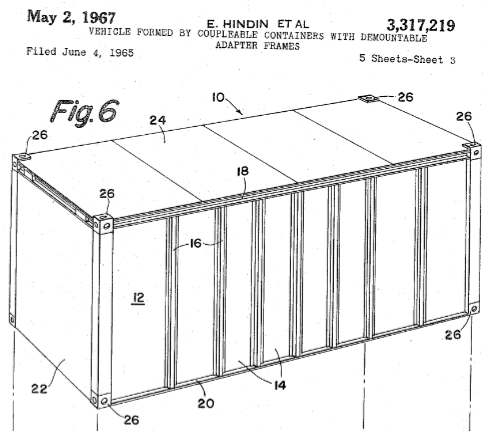
\includegraphics[width=70mm]{images/container_patent.png}
  \end{figure}
\end{frame}

\begin{frame}{Containers}{Qual problema resolve no mundo físico?}
  \begin{figure}[ht!]
    \centering
    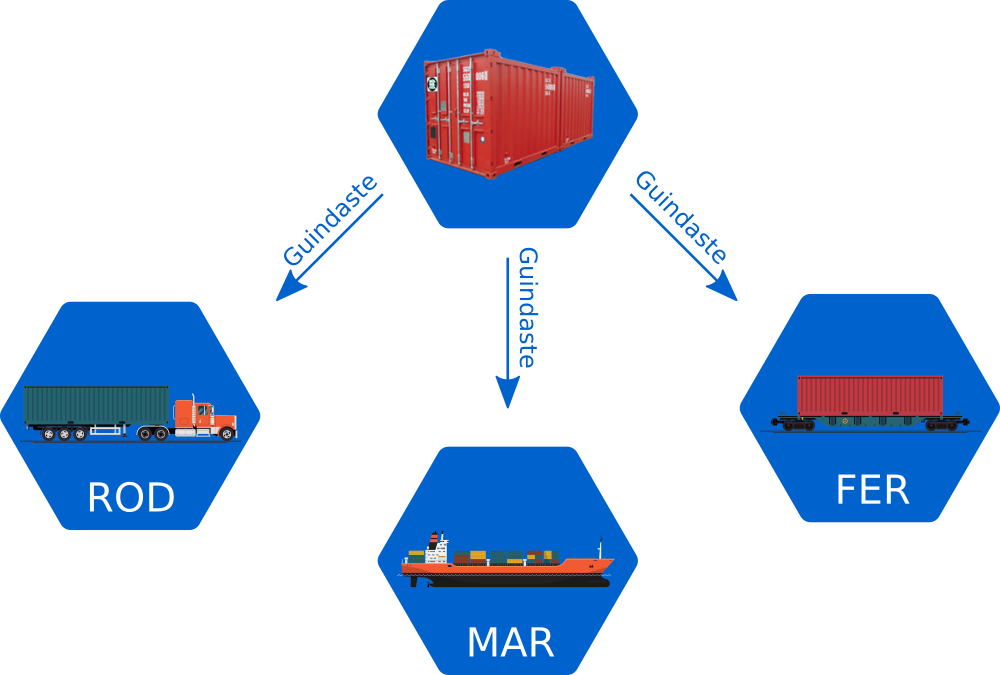
\includegraphics[width=95mm]{images/container_intermodal.png}
  \end{figure}
  \begin{center}
    CONTROLE > AGILIDADE > PORTABILIDADE
  \end{center}
\end{frame}

\subsection{No mundo digital}
\begin{frame}{Containers}{Qual problema resolve no mundo digital?}
 \begin{figure}[ht!]
    \centering
    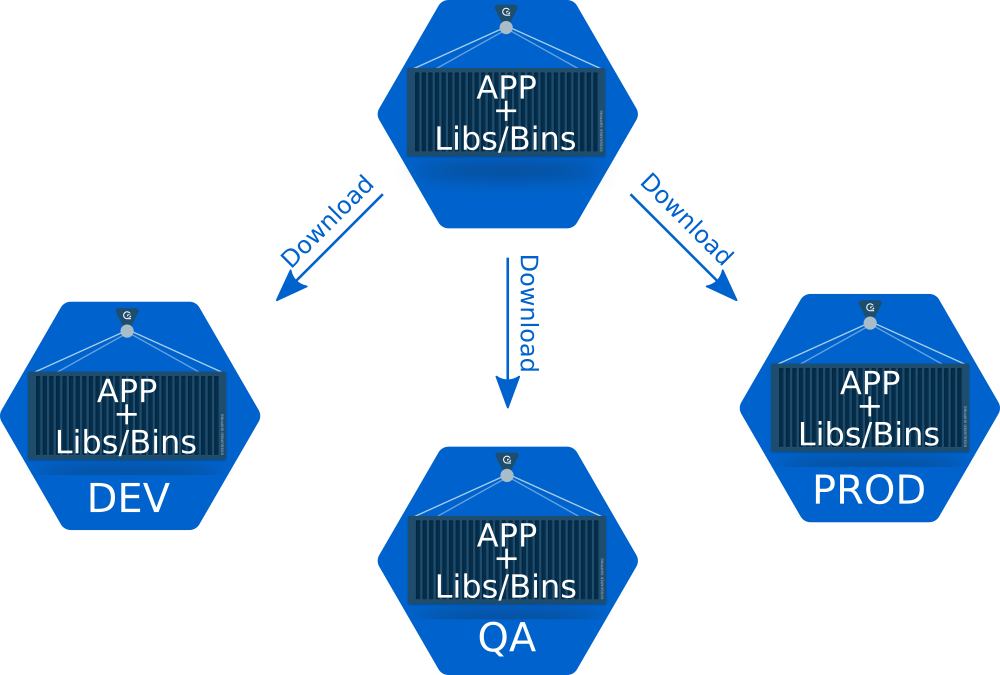
\includegraphics[width=95mm]{images/container_application.png}
  \end{figure}
  \begin{center}
    CONTROLE > AGILIDADE > PORTABILIDADE
  \end{center}
\end{frame}

\subsection{Timeline}
\begin{frame}{Containers}{Timeline}
  \begin{table}
    \centering
    \begin{minipage}[t]{.9\linewidth}
      \color{gray}
      \rule{\linewidth}{1pt}
      \ytl{1979}{Unix}{Chroot}
      \ytl{2000}{FreeBSD}{Jails}
      \ytl{2001}{Linux}{Linux-VServer}
      \ytl{2005}{Parallels}{OpenVZ Open Virtuozzo}
      \ytl{2006}{Google}{Control Groups}
      \ytl{2008}{Linux}{(LXC) Linux containers}
      \ytl{2013}{dotClould}{Docker}
      \ytl{2015}{OCI}{Docker e CoreOS}
      \ytl{2016}{Microsoft}{Windows Containers}
      \bigskip
      \rule{\linewidth}{1pt}
    \end{minipage}
  \end{table}
\end{frame}
